\chapter{From Bloom filters to Bloomaps}

During dataflow analysis the datastructure is almost as important as the
algorithm used. In the case of GCC, the structure chosen is a simple linked
list. This works fine for small data, but not so well with large data.

It is easy to convert the algorithm to a better data structure, but what do we
have to choose from? We already know the linked list can do all of that,
tree-like data structures, hash tables and many others could do all of those
things, but do the fit the profile of ideal data structure?

We will start by examining the needs of a typical Andersen-style algorithm and
comparing theoretical complexities of various well known data structures. In the
rest of this chapter we will describe a new enhancement of bloom filters called
Bloomaps.

\section{Requirements}

We need a data structure holding sets of integers, that is compact nad has the
following operations: {\tt INSERT}, {\tt QUERY}, {\tt INTERSECT} and {\tt
ENUMERATE} and {\tt UNION}; each of them with a specific purpose:

\begin{itemize}
	\item The {\tt INSERT} operation is called only at the initialization.
	\item The {\tt QUERY} operation is mostly called for a few special values,
		and they can be handled separately, or at the end.
	\item the {\tt INTERSECT} operation is called at the end, to answer alias
		oracle queries.
	\item The {\tt UNION} operation is called many times in each iteration, for
		every dependency on a changed set.
	\item The {\tt ENUMERATE} operation is called only on pointer dereference.
\end{itemize}

In other words, the basic operations can be a bit slower, but we need a good and
fast {\tt UNION}.

There a few other considerations:

\begin{itemize}
	\item The {\tt UNION} will be called on the same pairs over and over again,
		which means most of the elements will be already in both.
	\item The average number of stored elements will be small, and the data sparse.
\end{itemize}

A simple bitmap is a straightforward solution, but the parseness make it
unviable. Many tree-like structures will have problems with the intersections,
as all the elements have to examined and deduplicated.

A natural choice is a bloom filter, which is compact and has a fast union. The
compactness is a real treat, as we can go as far as to choose how much memory to
invest and sacrifice the precision if we don't have enough. Unfortunately, its
performance in {\tt INTERSECT} is rather suboptimal, and even worse, completely
lacks the {\tt ENUMERATE} operation.


\section{Bloom filters}

A bloom filter is a classical probabilistic data structure, invented by Burton
Howard Bloom in 1970 [REF:Bloom1970]. The goal is to provide a data structure
that has some nonzero probability of {\it false-positive}, but zero probability
of{\it false-negative}. This is accomplished by taking a bit field of $m$ bits,
$k$ hash functions, and hashing every element into $k$ different bits, writing
$1$ on insertion, and checking if every position contains $1$ on query.

The Bloom filter has immediate applications in some areas, for example caching:
it's a good idea to ask a filter if an element is in the cache. If the answer is
no, we need to get it elsewhere. If the answer is yes, we can look into the
cache, and in the worst case it's not there (an ocurrence false-positive).

Here is a short list of properties (provided the hashes can be computed in
constant time, which is often possible).:

\begin{itemize}
	\item {\tt QUERY} in $\O(1)$ time.
	\item {\tt INSERT} in $\O(1)$ time.
	\item {\tt DELETE, ENUMERATE, RESIZE} not supported.
	\item {\tt UNION} in $\O(m)$ time (bitwise OR).
	\item {\tt INTERSECTION} in $\O(m)$ time (bitwise AND).
\end{itemize}

To be honest, the last one is bit of a lie, as it's not an intersection as one
would expect. Let's denote $BF(A)$ as a bloom filter created from empty filter
by inserting elements from $A$ one by one. Then:

For $A,B$ it does not hold that $BF(A \cap B) = BF(A) \cap
BF(B)$. Unfortunately, even the inequation $BF(A \cap B) \subseteq BF(A) \cap
BF(B)$ holds, it's nowhere near the equality. Most imporantly, we would like to
check for emptyness of intersection, which is hard to achieve.

\section{Bloom filter intersection}

Although a bloom filter intersection easily computed with bitwise {\tt AND},
it's rarely accurate. The basic properties are already understood:

As proven by {\it Guo et. al.} [REF:Guo10], the probability that $BF(A\cap B) =
BF(A) \cap BF(B)$ is:
\begin{align}
p = (1-1/m)^{k^2\cdot |A-A\cap B| \cdot |B - A\cap B|}
\end{align}

For set emptyness, we can further simplify the formula by separating two cases:
$|A \cap B| > 0$ and $|A \cap B| = 0$. The first case is not interesting, the
second one however is:

Assuming that $A\cap B$ is empty, let's compute the probability that $BF(A) \cap
BF(B)$ is also empty.
\begin{align}
	p_{empty} = (1-1/m)^{k^2 \cdot |A| \cdot |B|}
\end{align}

Furthermore, if we use partitioned Bloom filters, Jeffrey and Steffan
[REF:Jeffrey11] showed a slightly improved probability:
\begin{align}
	p_{empty} = \left(1 - \left( 1 - {k \over m}\right)^{|A|\cdot |B|}\right)^k
\end{align}

This is due to the fact that it's enough to have one empty partition to consider
the filter empty, as every query would result in false in the empty partition.

However, in the same article they proved that pure Bloom filter intersection is more
memory-consuming than more conventional queue-of-queries. In the next section,
a hybrid solution is provided that can be used with both of these approaches,
based on the time requirements.

\section{Bloom filter enumeration}

It's immediately clear that vanilla Bloom filter cannot provide list of it's
possible elements, as for example the simplest filter holding $1$ elements and
answering with false-positive probability $0.5$ would have to enumerate half the
universe $U$.

Besides the trivial queue-of-queries, there has been one attempt at constructing
Bloom filter-like structure, that can list it's items, the Invertible Bloom
Lookup Tables, by Michael T. Goodrich [REF:Goodrich11]. The problem of IBLT is
that they have non-zero probability of being unable to produce a complete list
of entries, and do not provide the advantages of classic Bloom filters, as a
fast intersection and membership queries. This said, we will not attempt to use
them, although they are perhaps an interesting structure for future work.

Let us review in short the available methods:

\paragraph{Enumerate entire universe.} This is possible for $U$ small enough
\paragraph{Keep a Queue-of-queries for each filter.} Perhaps the most sensible
way, if there are either few filters, or only a few elements in each filter.
\paragraph{Keep a single Queue-of-queries for all filter.}

Every one of these approaches has it's use case. We will provide a similar
approach, suitable for relatively small, but possibly sparse universe, avoiding
most of the overhead caused by queues-of-queries. This approach assumes that
32bit integers are being stored, represeting large number of sets.

\section{Bloomaps and Families}

\paragraph{Definition.} Bloomap Family with parameters $(m, k, s)$ is a
datastructure that maintains a list of Bloomaps of the same parameters, and
indexed representation of used parts of the universe in union of all it's
Bloomaps, capable of enumeration.

\paragraph{Definition.} Bloomap is an enhanced Bloom filter, belonging to a single
family, capable of executing {\tt INSERT} and {\tt QUERY} itself, and {\tt
ENUMERATE}, {\tt UNION} and {\tt INTERSECT} within it's family.

A bloomap with parameters $(m, k, s)$ is constructed from a partitioned Bloom
filter with the addition of a {\it side index} containing $s$ bits. The side
index is used as another partition in the bloomfilter, however with simpler hash
function that is easily inverted (for example a simple {\tt SHIFT} and {\tt
AND} with a mask).

Furthermore, the Bloomaps and their families need to fulfill these conditions:

\begin{itemize}
	\item When a new item is inserted into a Bloomap, it is also inserted into
		the family.
	\item A Family has to enumerate all items inserted into it's Boomaps for any
		given hash.
\end{itemize}

Let's take a look on how these data structures might look in pseudocode (based
on C++):


\begin{verbatim}
struct Bloomap {
    BloomapFamily f;
    int m,k,s;

    int index[s];
    int partitions[k][m/k];
};

struct BloomapFamily {
    vector Bloomap;
    int m,k,s;

    hash_set universe;
}
\end{verbatim}

Where {\tt hash\_set} is some data structure capable of storing a set of
elements from universe associated with a given hash. The naive C++ structure
might be {\tt hash\_map<vector<universe\_type>>}.

Before we get into technicalities, let's illustrate how {\tt INSERT} and {\tt
ENUMERATE} functions might be implemented:

\begin{verbatim}
function INSERT(bloomap,element) {
    # Decompose element into offset, index_hash and data.
    (offset,index_hash,data) := element;
    # Insert into side_index of a bloomap.
    index[index_hash] := true;
    for (i := 1..k) {
        partitions[i][hash(i,element) % m/k] := 1
    }
    # Insert into universe index of a family
    f.universe[hash] += element;
}

function ENUMERATE(bloomap) {
    list = ();
	for (i := 1..s | index[i] == true) {
        for (element in f.universe[i] | element in bloomap) 
            list += element;
    }
    return list;
}
\end{verbatim}

Both of them are pretty straightforward, as {\tt INSERT} is a regular function
for Bloom filter insertion, with the added partition fo side index and family
universe insertion.

We might expect this to run in $\O(1)$, as it does for Bloom filters. Writing to
the index doesn't make it worse, but inserting into a universe might. Depending
on the set implementation, we can expect additional $\O(\log n)$ for tree-based
implementations or amortized $\O(1)$ for hash-based implementations. We probably
can't do much better in generic case, but we will suggest a worst-case $\O(1)$
for reasonable integers (dense sequence of ids starting from 0).


\subsection{Compact representation of dense integer universe}

Representing universe requires storing sets for different hashes. It's wasteful
to store them in a linked-list, trees or even hash tables, as a humble bit array
fulfills the task. A little unusual form of a bit array has been used, in order
to achieve less allocations and space efficiency.

As mentioned above, we will split the value to {\tt offset}, {\tt hash} and {\tt
data} at binary boundaries. This means we can simply concatenate the values to
get the represented integer, and vice versa. We can now organize the data into
{\it buckets} and {\it superbuckets} in the following way:

\begin{itemize}
	\item Each offset has it's own {\it superbucket}.
	\item Each {\it superbucket} contains a {\it bucket} for every {\tt hash} value.
	\item Each {\it bucket} contains a bit for every {\tt data} value.
\end{itemize}

In this way a bit corresponding to an element can be easily found, and vice
versa.

\begin{center}
	{\tt element = offset$\cdot$hash$\cdot$data} $\Leftrightarrow$
	{\tt universe[offset$\cdot$hash].bit[data]}
\end{center}


\begin{figure}[h!]
	\centering
	\label{figure-bucketshop}
	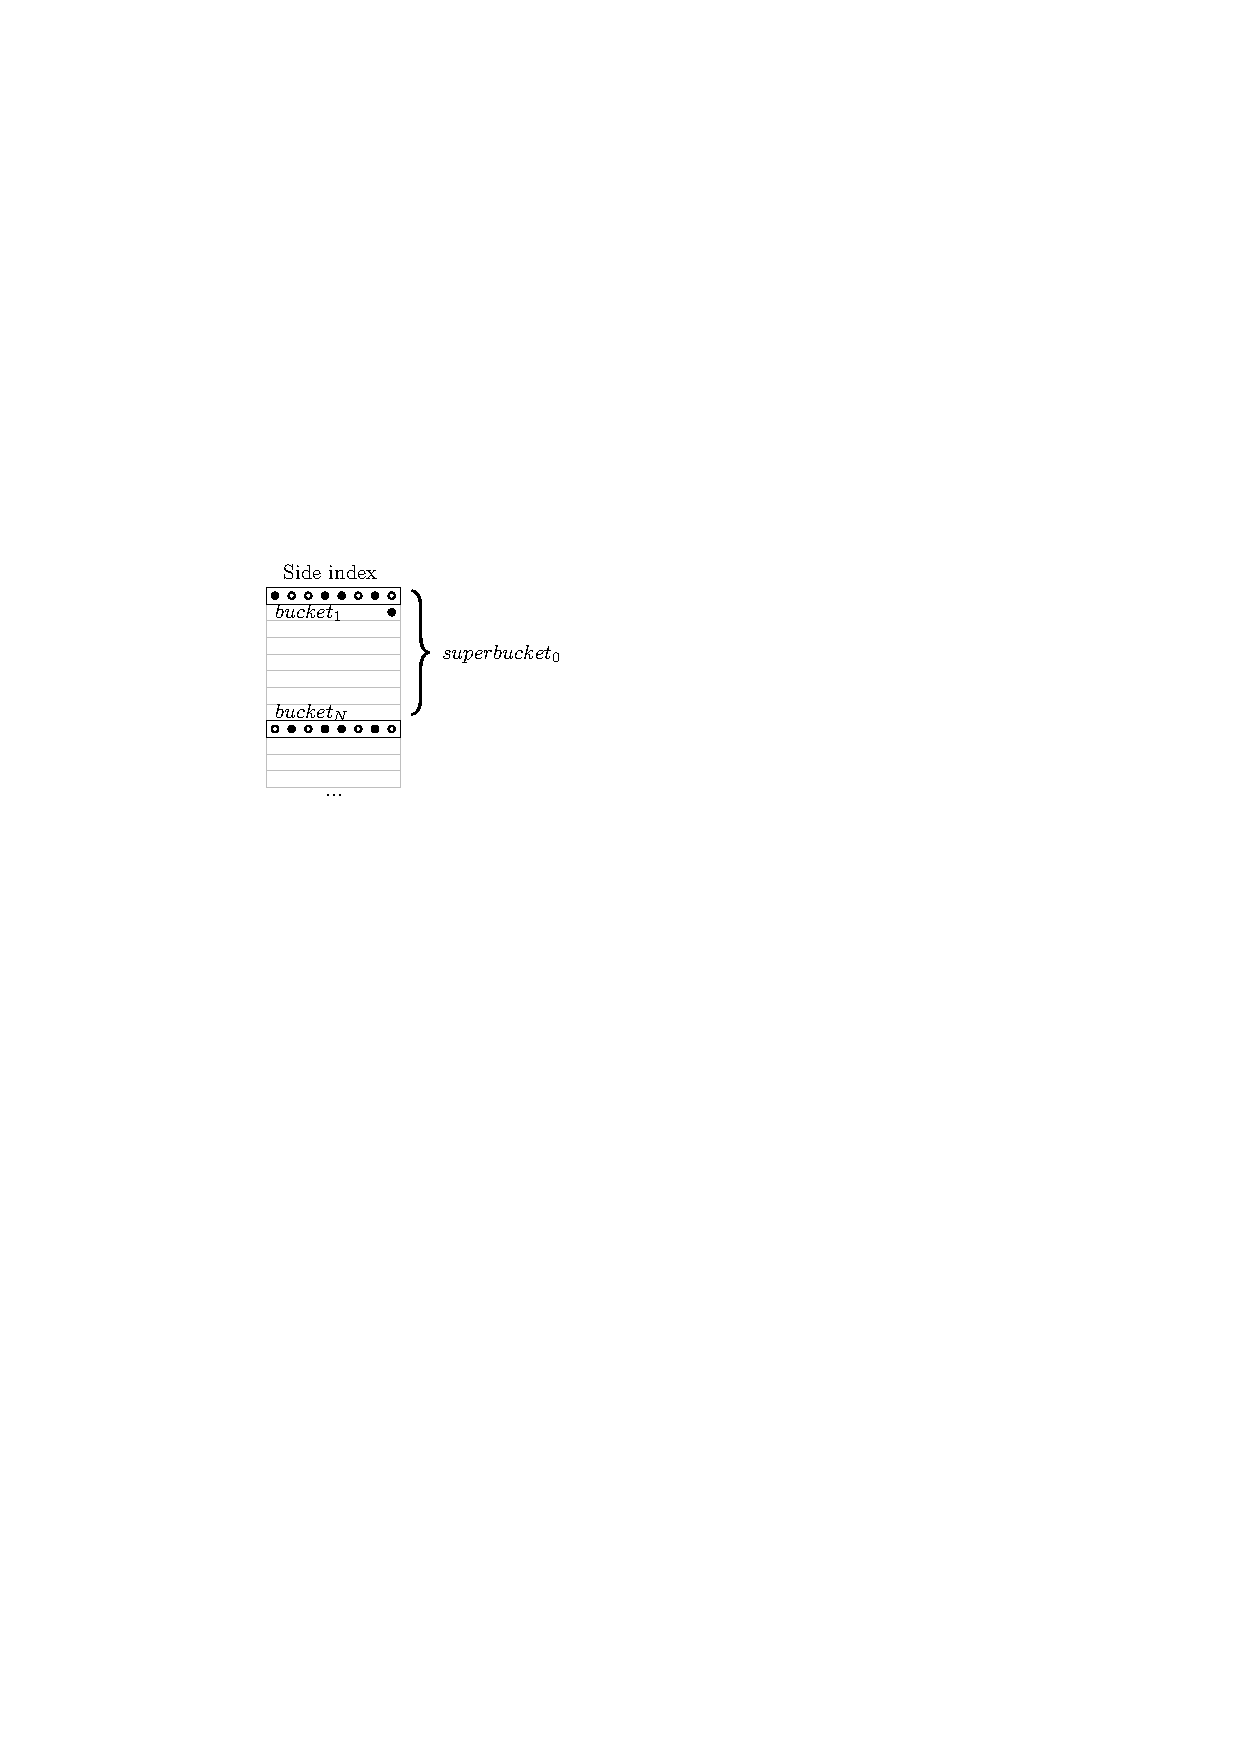
\includegraphics{img/bucketshop.pdf}
	\caption{Bucket and superbuckets in an array}
\end{figure}
